\documentclass[english, ngerman]{beamer}
\usepackage[T1]{fontenc} %% T1 encodierte Schriften laden, da diese
                       %% Umlaute als eingene Zeichen enthalten und
                       %% so die Worttrennung automatisch funktioniert
\usepackage{umlaut}    %% Das � wird vom fontenc Package nicht erkannt,
                       %% aber vom Umlaut Package
                    
\usepackage{babel}     %% Ist wichtig f�r die Umsetzung von \section
                       %% etc. in die jeweilige Sprache 

\mode<presentation>
{
  	\usetheme{Warsaw}
        \setbeamercovered{dynamic}
        \setbeamertemplate{background canvas}[vertical shading][bottom=red!10,top=blue!10]
        \usefonttheme[onlysmall]{structurebold}
}
\usepackage[latin1]{inputenc}
\usepackage{hyperref}
\usepackage{graphicx}
\usepackage{amsmath}
\usepackage{times}
\usepackage{pgf,pgfarrows,pgfnodes,pgfautomata,pgfheaps,pgfshade}

\title[Rock'n'Roll, a Engine for ``EinStein W�rfelt Nicht''\texttrademark]{
  Rock'n'Roll\\
  A Engine for the Board Game\\
  ``EinStein W�rfelt Nicht''\texttrademark
}

\author{Andreas Sch�fer}
\date{June 13, 2006}
\institute[FSU Jena]{
  Institut f�r Informatik\\
  Friedrich-Schiller-Universit�t Jena
}


\begin{document}

\frame{\titlepage}

\section*{Outline}

\begin{frame}
  \frametitle{Outline}
  \tableofcontents[pausesections]
\end{frame}

\AtBeginSubsection[]
{
  \begin{frame}
    \frametitle{Outlook}
    \tableofcontents[current,currentsubsection]
  \end{frame}
}

\section{Introduction to EinStein}

\subsection{The Rules}

\begin{frame}
  \begin{columns}
    \column{8.5cm}    
    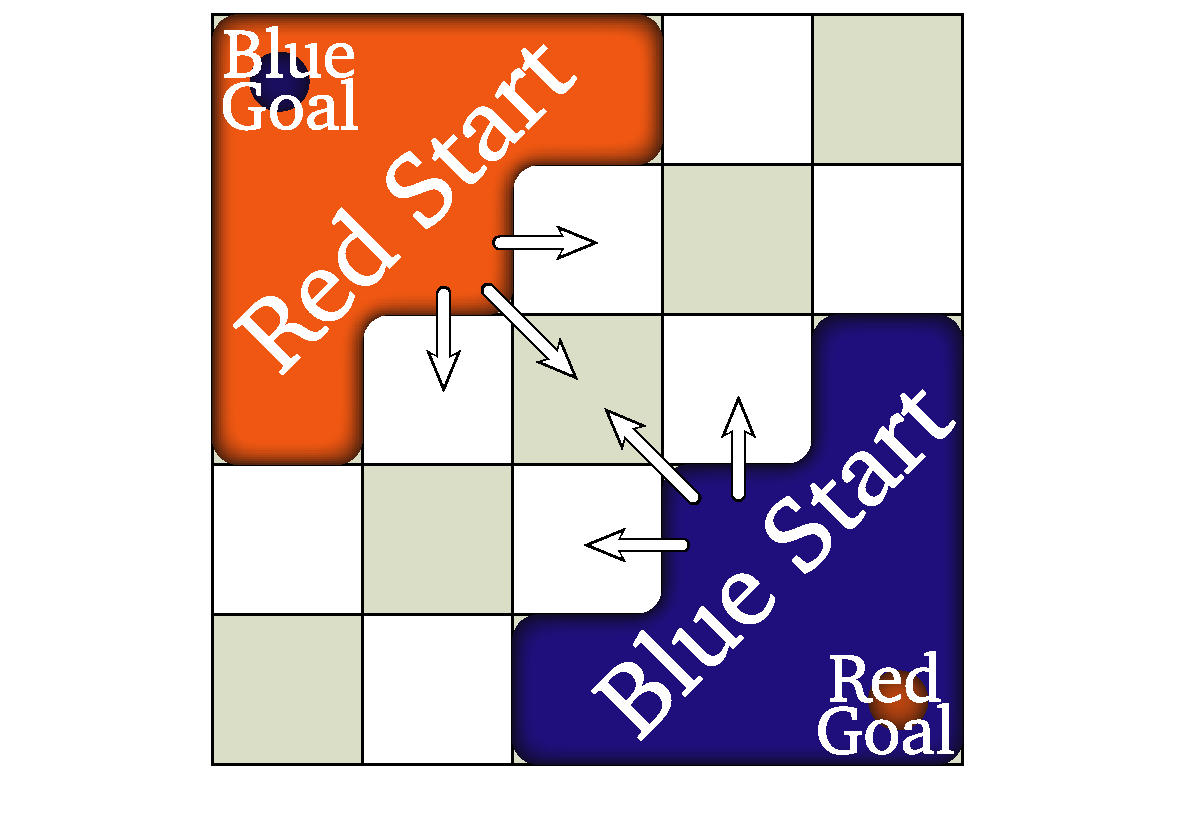
\includegraphics[scale=0.5]{board_setup}    
    \column{5cm}    
    Objective:
    \begin{itemize}
    \item reach goal or
    \item capture every of the opponent's stones
    \end{itemize}
  \end{columns}
\end{frame}

\begin{frame}
  \begin{columns}
    \column{8.5cm}    
    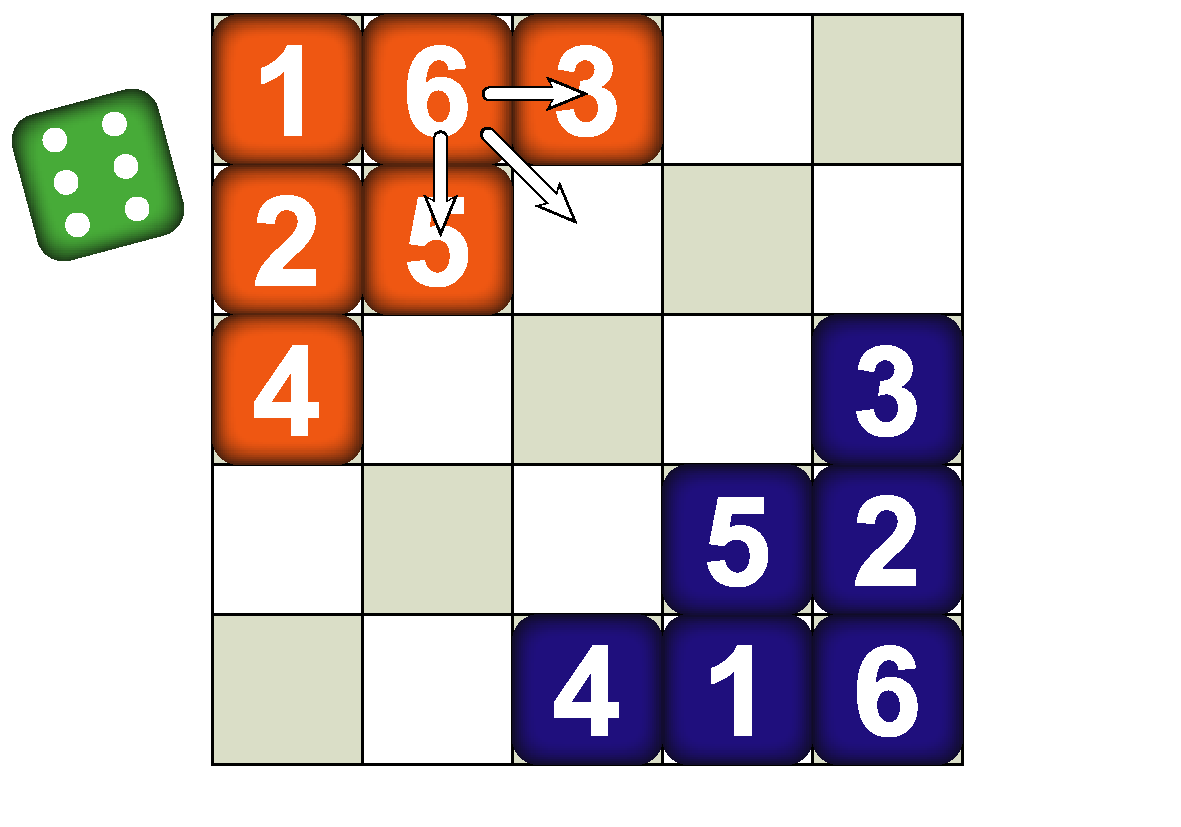
\includegraphics[scale=0.5]{board_start}    
    \column{5cm}    
    \begin{enumerate}
    \item players take turns
    \item dice determines\\
      which stone to move
    \item self capturing\\is legal
    \end{enumerate}
  \end{columns}
\end{frame}

\begin{frame}
  \begin{columns}
    \column{8.5cm}    
    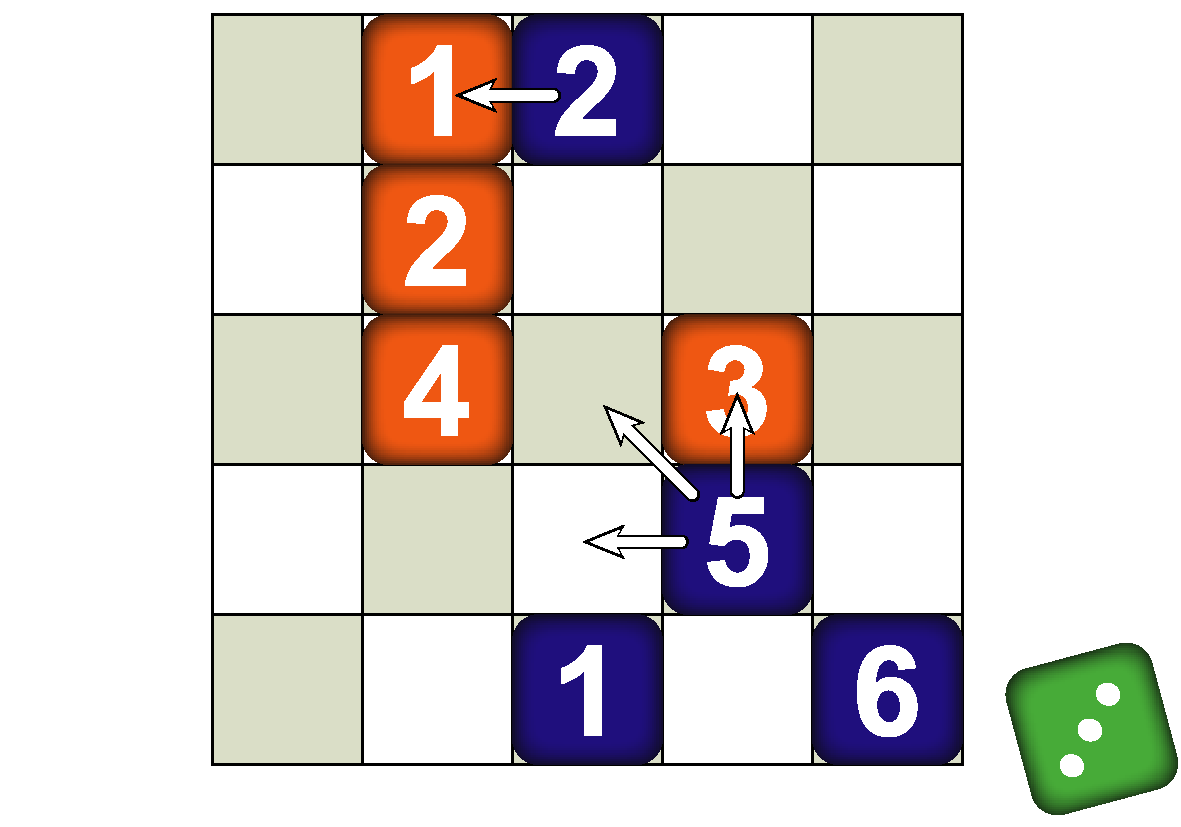
\includegraphics[scale=0.5]{board_med}    
    \column{3.5cm}    
    \begin{block}{}
      If the rolled number\\ 
      is missing then an\\
      adjacent stone has\\
      to be moved      
    \end{block}
    \column{1.5cm}
  \end{columns}
\end{frame}

\begin{frame}
  \begin{columns}
    \column{8.5cm}    
    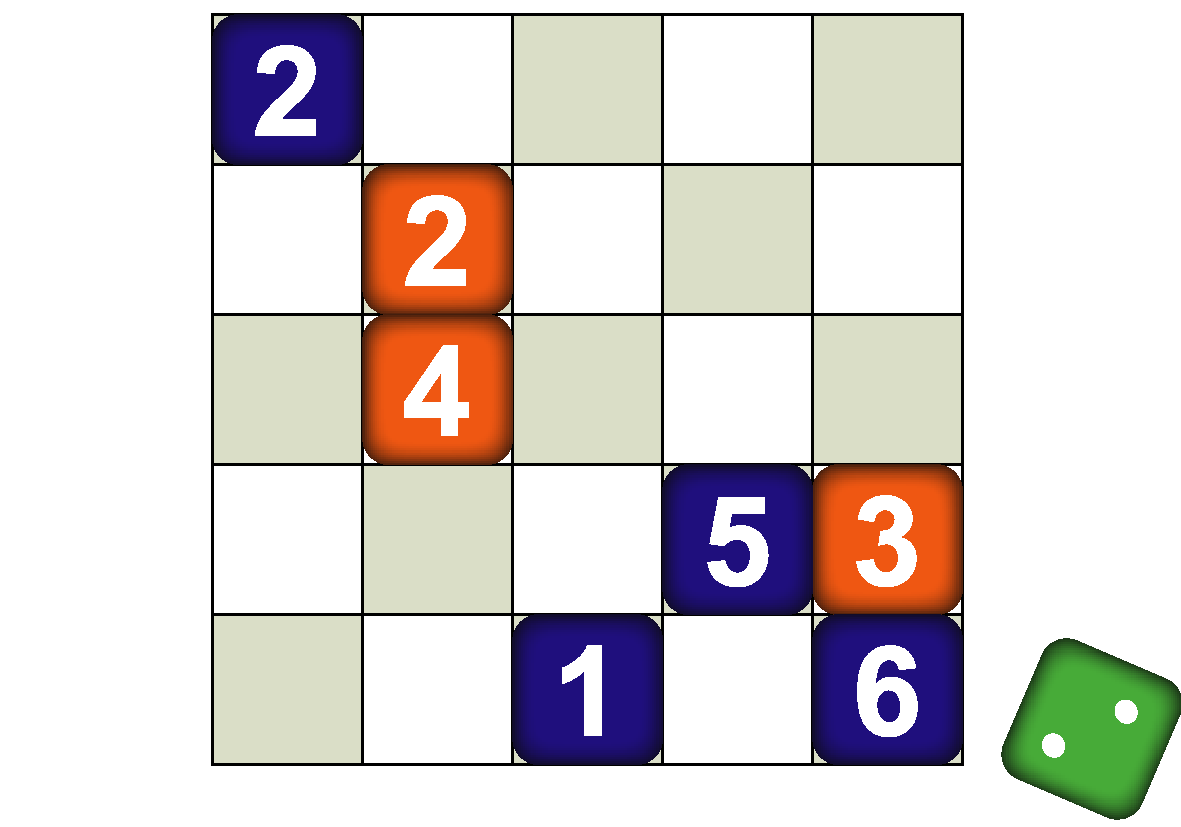
\includegraphics[scale=0.5]{board_end}    
    \column{5cm}    
    Blue won by reaching\\
 his goal
  \end{columns}
\end{frame}

\section{Engine Algorithms}

\subsection{Heuristics}

\begin{frame}
  \frametitle{Heuristics}
  \begin{itemize}
  \item heuristic = rule of thumb,
  \item computer needs to choose \emph{good} moves,
  \item heuristic maps boards to the reals,
  \item good boards \emph{hopefully} get higher ratings
  \end{itemize}
\end{frame}

\begin{frame}
  \frametitle{Schwarz Tables}
  \begin{columns}
    \column{8cm}
    \begin{itemize}
    \item estimate for each player,\\
      how many moves excepted\\
      to reach goal
    \item difference of the two estimates\\
      is the board rating
    \item capturing is ignored

    \end{itemize}

    \column{4cm}
    Example:\\(
    one player only)
    \begin{pgfpicture}{0cm}{0cm}{3.425cm}{3.425cm}
      \color{black!25}
      \pgfmoveto{\pgfxy(2.74,0.0)}
      \pgflineto{\pgfxy(3.425,0.0)}
      \pgflineto{\pgfxy(3.425,0.685)}
      \pgflineto{\pgfxy(2.74,0.685)}
      \pgfclosepath
      \pgffill
      \color{black}
      \pgfxyline(0.0,0)(0.0,3.425)
      \pgfxyline(0.685,0)(0.685,3.425)
      \pgfxyline(1.37,0)(1.37,3.425)
      \pgfxyline(2.055,0)(2.055,3.425)
      \pgfxyline(2.74,0)(2.74,3.425)
      \pgfxyline(3.425,0)(3.425,3.425)
      \pgfxyline(0,0.0)(3.425,0.0)
      \pgfxyline(0,0.685)(3.425,0.685)
      \pgfxyline(0,1.37)(3.425,1.37)
      \pgfxyline(0,2.055)(3.425,2.055)
      \pgfxyline(0,2.74)(3.425,2.74)
      \pgfxyline(0,3.425)(3.425,3.425)
      \pgfputat{\pgfxy(1.7125,3.0825)}{\pgfbox[center,center]{4}}
    \end{pgfpicture}
    remaining moves = 4
  \end{columns}
\end{frame}

\begin{frame}
  \frametitle{Schwarz Tables (cont.)}
  Example 2:\\
  (again just one player)\\
  \begin{columns}
    \column{4cm}
    \begin{pgfpicture}{0cm}{0cm}{3.425cm}{3.425cm}
      \color{black!25}
      \pgfmoveto{\pgfxy(2.74,0.0)}
      \pgflineto{\pgfxy(3.425,0.0)}
      \pgflineto{\pgfxy(3.425,0.685)}
      \pgflineto{\pgfxy(2.74,0.685)}
      \pgfclosepath
      \pgffill
      \color{black}
      \pgfxyline(0.0,0)(0.0,3.425)
      \pgfxyline(0.685,0)(0.685,3.425)
      \pgfxyline(1.37,0)(1.37,3.425)
      \pgfxyline(2.055,0)(2.055,3.425)
      \pgfxyline(2.74,0)(2.74,3.425)
      \pgfxyline(3.425,0)(3.425,3.425)
      \pgfxyline(0,0.0)(3.425,0.0)
      \pgfxyline(0,0.685)(3.425,0.685)
      \pgfxyline(0,1.37)(3.425,1.37)
      \pgfxyline(0,2.055)(3.425,2.055)
      \pgfxyline(0,2.74)(3.425,2.74)
      \pgfxyline(0,3.425)(3.425,3.425)
      \pgfputat{\pgfxy(3.0825,1.7125)}{\pgfbox[center,center]{6}}
      \pgfputat{\pgfxy(2.3975,1.0275)}{\pgfbox[center,center]{1}}
    \end{pgfpicture}
    \column{6cm}
    remaining moves $= \frac{5}{6} \cdot 1 + \frac{1}{6} \cdot 2 = \frac{7}{6}$
  \end{columns}
\end{frame}

\subsection{Minimax}

\begin{frame}
  \frametitle{Basic Minimax}
  \begin{columns}
    \column{7.5cm}
    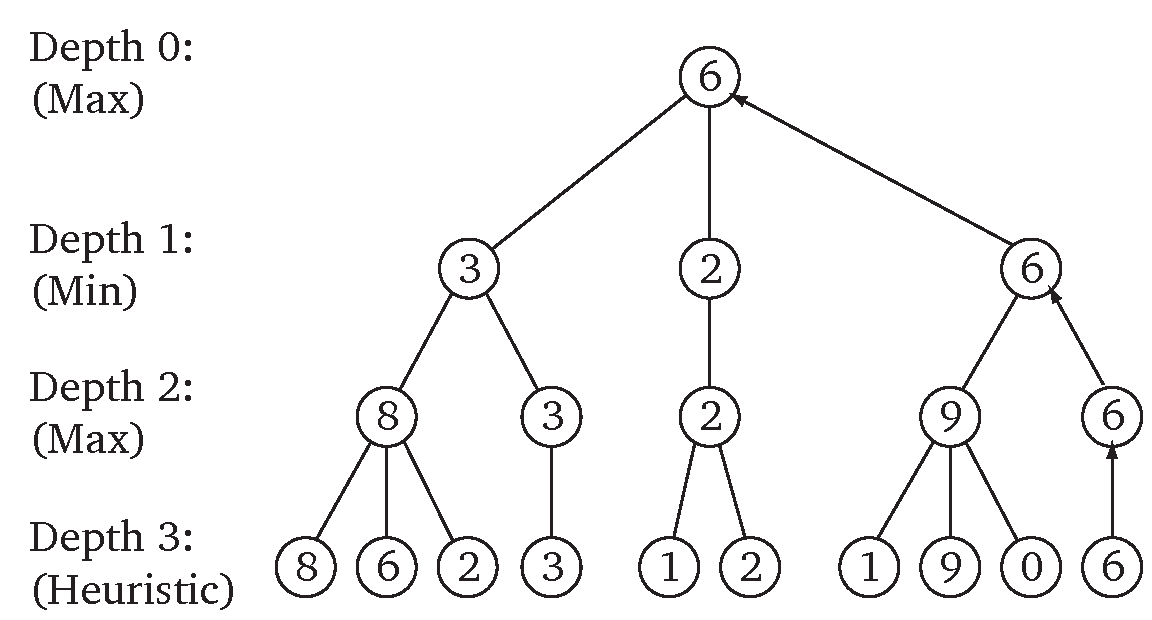
\includegraphics[scale=0.4]{treesearchBasics}
    
    \column{6cm}
    \begin{itemize}
    \item look some moves ahead
    \item cut at a given depth and assign ratings
    \item two players: 
      \begin{itemize}
      \item Max tries to \emph{maximize},
      \item Min tries to \emph{minimize}
      \end{itemize}
      \item propagate values upwards
    \end{itemize}

  \end{columns}
\end{frame}

\begin{frame}
  \frametitle{Basic Minimax (cont.)}
  \begin{columns}
    \column{7.5cm}
    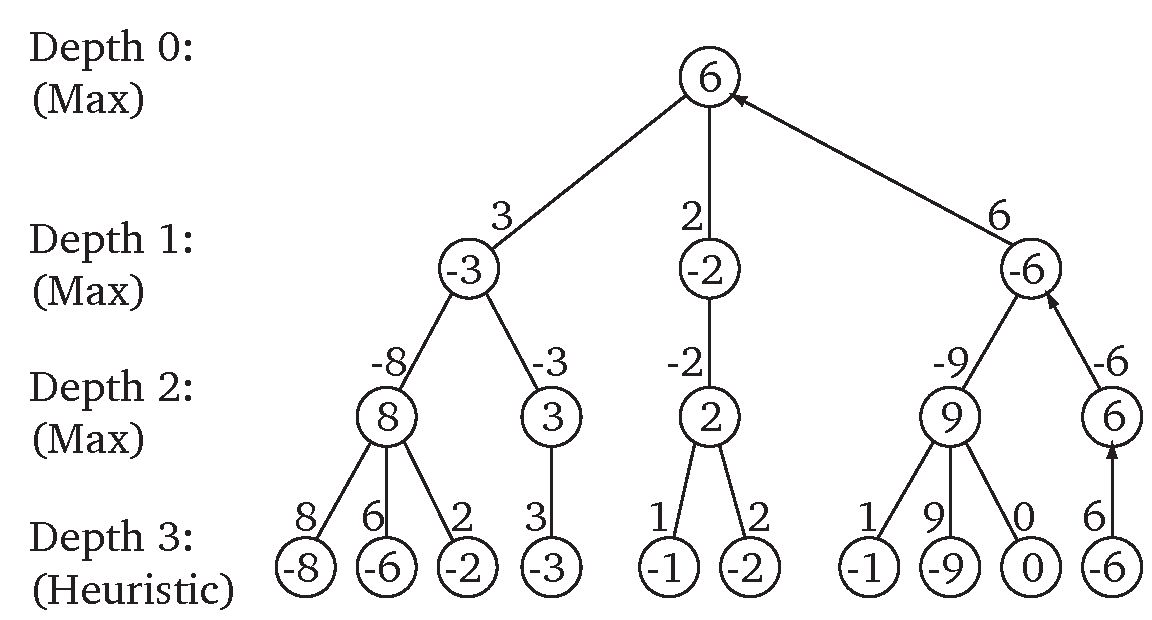
\includegraphics[scale=0.4]{treesearchMaxOnly}
    
    \column{6cm}
    Simplification: 
    \begin{itemize}
    \item invert values before propagation
    \item only maximizing nodes necessary
    \end{itemize}
  \end{columns}
\end{frame}

\begin{frame}
  \frametitle{Expect Minimax}
  \begin{itemize}
  \item problem: EinStein is randomized
  \item standard solution: introduction of dicing layers
  \item problem: much redundant evaluations
  \end{itemize}
  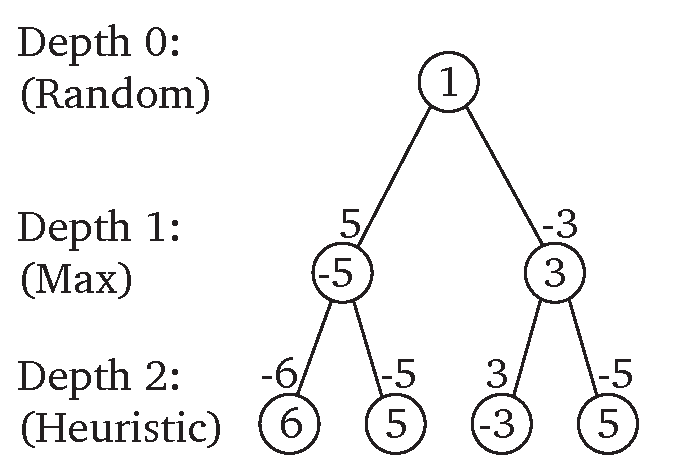
\includegraphics[scale=0.4]{treesearchRandomLayers}
\end{frame}


\begin{frame}
  \frametitle{Dicing Layer Reduction}
  Unified Operator avoids unnecessary evaluations:
  \begin{itemize}
  \item calculate for each stone $i$ the best move $r_i$ 
  \item determine for each stone $i$ probability $p_i$  to be moved 
  \item rating $ R = \sum\limits_{i=1}^{6} r_ip_i$
  \end{itemize}
  \begin{center}
    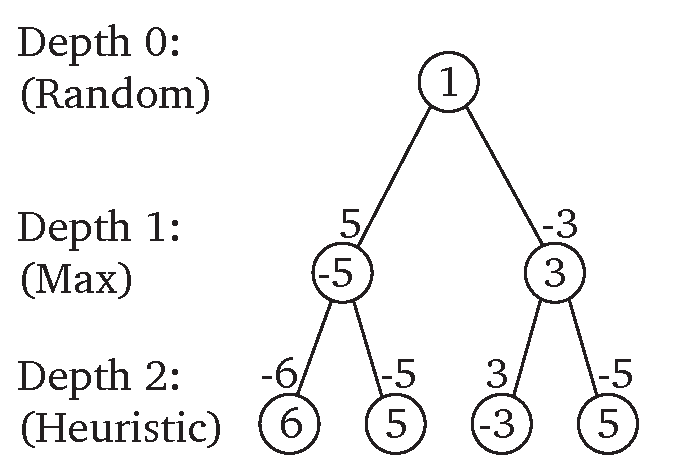
\includegraphics[scale=0.4]{treesearchRandomLayers}
    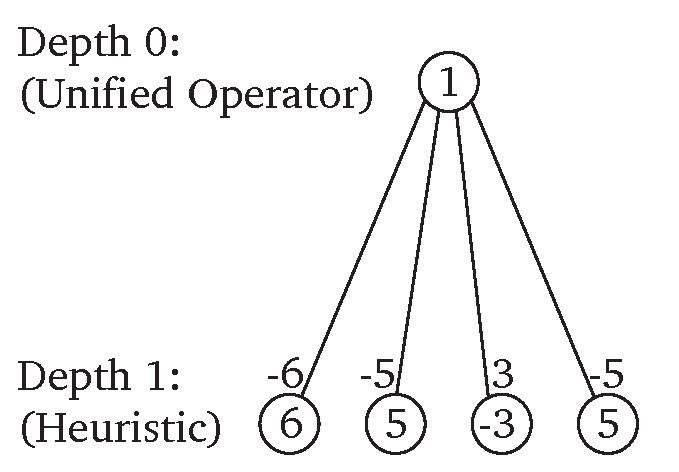
\includegraphics[scale=0.4]{treesearchRandomLayersGone}  
  \end{center}
\end{frame}

\subsection{Monte Carlo Method}

\begin{frame}
  \frametitle{The Monte Carlo Method}
  \begin{block}{board evaluation:}
    \begin{itemize}
    \item 2 simple players finish game (e.g. simple heuristic)
    \item many repeats (e.g. 200 times)
    \item hopefully: win/loose ratio is correlated to move quality
    \item improved long-term foresight
    \item worse short-term foresight
    \end{itemize}   
  \end{block}
\end{frame}

\section{Benchmarks}

\subsection{Best Parameter Sets}

\begin{frame}
  \frametitle{Monte Carlo vs. Minimax}
  \begin{tabular}{ll|rrrrrrr}
    & Player & 1    & 2    & 3    & 4    & 5    & 6    & 7\\  
    \hline
    1 & Random(1)                        & \multicolumn{1}{c}{--} & 11 &  9 & 10 &  7 &  7 &  7 \\
    2 & Monte(1,\ \ \ 50, Schwarz(1))    & 88 & \multicolumn{1}{c}{--} & 45 & 55 & 44 & 41 & 40 \\
    3 & Monte(1,        200, Schwarz(1)) & 91 & 55 & \multicolumn{1}{c}{--} & 62 & 49 & 46 & 45 \\
    4 & Schwarz(1)                       & 90 & 44 & 38 & \multicolumn{1}{c}{--} & 41 & 40 & 39 \\
    5 & Schwarz(5)                       & 93 & 55 & 51 & 59 & \multicolumn{1}{c}{--} & 47 & 46 \\
    6 & Monte(3, 20, Farmer(1))          & 93 & 59 & 54 & 60 & 53 & \multicolumn{1}{c}{--} & 50 \\
    7 & Monte(3, 40, Farmer(1))          & 93 & 60 & 55 & 61 & 54 & 50 & \multicolumn{1}{c}{--} \\
%     1 & Random(0)                        & \multicolumn{1}{c}{--} & 11.0 &  8.6 & 10.0 &  7.0 &  6.8 &  6.9 \\
%     2 & Monte(0,\ \ \ 50, Schwarz(0))    & 88.9 & \multicolumn{1}{c}{--} & 45.0 & 55.9 & 44.7 & 41.2 & 40.3 \\
%     3 & Monte(0,        200, Schwarz(0)) & 91.4 & 54.9 & \multicolumn{1}{c}{--} & 61.8 & 49.2 & 46.2 & 45.0 \\
%     4 & Schwarz(0)                       & 89.9 & 44.0 & 38.1 & \multicolumn{1}{c}{--} & 41.2 & 40.3 & 39.1 \\
%     5 & Schwarz(4)                       & 92.9 & 55.2 & 50.7 & 58.7 & \multicolumn{1}{c}{--} & 47.3 & 45.5 \\
%     6 & Schwarz(2, 20, Farmer(0))        & 93.1 & 58.7 & 53.8 & 59.6 & 52.6 & \multicolumn{1}{c}{--} & 49.9 \\
%     7 & Schwarz(2, 40, Farmer(0))        & 93.0 & 59.6 & 54.9 & 60.8 & 54.4 & 50.0 & \multicolumn{1}{c}{--} \\
  \end{tabular}    
    \begin{block}{}
    \begin{itemize}
    \item Schwarz(n) = Minimax with depth n and Schwarz Tables
    \item Monte(n, r, p) = Minimax with depth n and subsequent Monte Carlo (r repeats and p as simulation players)
    \end{itemize}    
  \end{block}
\end{frame}

\subsection{Optimal Starting Position}

\begin{frame}
  \frametitle{Optimal Starting Positions}
  \begin{tabular}{ccc}
  \begin{pgfpicture}{0cm}{0cm}{3.425cm}{3.425cm}
    \color{black!25}
    \pgfmoveto{\pgfxy(2.74,0.0)}
    \pgflineto{\pgfxy(3.425,0.0)}
    \pgflineto{\pgfxy(3.425,0.685)}
    \pgflineto{\pgfxy(2.74,0.685)}
    \pgfclosepath
    \pgffill
    \color{black}
    \pgfxyline(0.0,0)(0.0,3.425)
    \pgfxyline(0.685,0)(0.685,3.425)
    \pgfxyline(1.37,0)(1.37,3.425)
    \pgfxyline(2.055,0)(2.055,3.425)
    \pgfxyline(2.74,0)(2.74,3.425)
    \pgfxyline(3.425,0)(3.425,3.425)
    \pgfxyline(0,0.0)(3.425,0.0)
    \pgfxyline(0,0.685)(3.425,0.685)
    \pgfxyline(0,1.37)(3.425,1.37)
    \pgfxyline(0,2.055)(3.425,2.055)
    \pgfxyline(0,2.74)(3.425,2.74)
    \pgfxyline(0,3.425)(3.425,3.425)
    \pgfputat{\pgfxy(0.3425,3.0825)}{\pgfbox[center,center]{6}}
    \pgfputat{\pgfxy(1.0275,3.0825)}{\pgfbox[center,center]{2}}
    \pgfputat{\pgfxy(1.7125,3.0825)}{\pgfbox[center,center]{4}}
    \pgfputat{\pgfxy(0.3425,2.3975)}{\pgfbox[center,center]{1}}
    \pgfputat{\pgfxy(1.0275,2.3975)}{\pgfbox[center,center]{5}}
    \pgfputat{\pgfxy(0.3425,1.7125)}{\pgfbox[center,center]{3}}
  \end{pgfpicture} &
  \begin{pgfpicture}{0cm}{0cm}{3.425cm}{3.425cm}
    \color{black!25}
    \pgfmoveto{\pgfxy(2.74,0.0)}
    \pgflineto{\pgfxy(3.425,0.0)}
    \pgflineto{\pgfxy(3.425,0.685)}
    \pgflineto{\pgfxy(2.74,0.685)}
    \pgfclosepath
    \pgffill
    \color{black}
    \pgfxyline(0.0,0)(0.0,3.425)
    \pgfxyline(0.685,0)(0.685,3.425)
    \pgfxyline(1.37,0)(1.37,3.425)
    \pgfxyline(2.055,0)(2.055,3.425)
    \pgfxyline(2.74,0)(2.74,3.425)
    \pgfxyline(3.425,0)(3.425,3.425)
    \pgfxyline(0,0.0)(3.425,0.0)
    \pgfxyline(0,0.685)(3.425,0.685)
    \pgfxyline(0,1.37)(3.425,1.37)
    \pgfxyline(0,2.055)(3.425,2.055)
    \pgfxyline(0,2.74)(3.425,2.74)
    \pgfxyline(0,3.425)(3.425,3.425)
    \pgfputat{\pgfxy(0.3425,3.0825)}{\pgfbox[center,center]{6}}
    \pgfputat{\pgfxy(1.0275,3.0825)}{\pgfbox[center,center]{5}}
    \pgfputat{\pgfxy(1.7125,3.0825)}{\pgfbox[center,center]{2}}
    \pgfputat{\pgfxy(0.3425,2.3975)}{\pgfbox[center,center]{1}}
    \pgfputat{\pgfxy(1.0275,2.3975)}{\pgfbox[center,center]{4}}
    \pgfputat{\pgfxy(0.3425,1.7125)}{\pgfbox[center,center]{3}}
  \end{pgfpicture} &
  \begin{pgfpicture}{0cm}{0cm}{3.425cm}{3.425cm}
    \color{black!25}
    \pgfmoveto{\pgfxy(2.74,0.0)}
    \pgflineto{\pgfxy(3.425,0.0)}
    \pgflineto{\pgfxy(3.425,0.685)}
    \pgflineto{\pgfxy(2.74,0.685)}
    \pgfclosepath
    \pgffill
    \color{black}
    \pgfxyline(0.0,0)(0.0,3.425)
    \pgfxyline(0.685,0)(0.685,3.425)
    \pgfxyline(1.37,0)(1.37,3.425)
    \pgfxyline(2.055,0)(2.055,3.425)
    \pgfxyline(2.74,0)(2.74,3.425)
    \pgfxyline(3.425,0)(3.425,3.425)
    \pgfxyline(0,0.0)(3.425,0.0)
    \pgfxyline(0,0.685)(3.425,0.685)
    \pgfxyline(0,1.37)(3.425,1.37)
    \pgfxyline(0,2.055)(3.425,2.055)
    \pgfxyline(0,2.74)(3.425,2.74)
    \pgfxyline(0,3.425)(3.425,3.425)
    \pgfputat{\pgfxy(0.3425,3.0825)}{\pgfbox[center,center]{1}}
    \pgfputat{\pgfxy(1.0275,3.0825)}{\pgfbox[center,center]{5}}
    \pgfputat{\pgfxy(1.7125,3.0825)}{\pgfbox[center,center]{4}}
    \pgfputat{\pgfxy(0.3425,2.3975)}{\pgfbox[center,center]{6}}
    \pgfputat{\pgfxy(1.0275,2.3975)}{\pgfbox[center,center]{2}}
    \pgfputat{\pgfxy(0.3425,1.7125)}{\pgfbox[center,center]{3}}
  \end{pgfpicture}\\
  56.056 \% & 56.021 \% & 55.913 \%\\
  \end{tabular}
\end{frame}

\begin{frame}
  \frametitle{Worst Starting Positions}
  \begin{tabular}{ccc}
    \begin{pgfpicture}{0cm}{0cm}{3.425cm}{3.425cm}
      \color{black!25}
      \pgfmoveto{\pgfxy(2.74,0.0)}
      \pgflineto{\pgfxy(3.425,0.0)}
      \pgflineto{\pgfxy(3.425,0.685)}
      \pgflineto{\pgfxy(2.74,0.685)}
      \pgfclosepath
      \pgffill
      \color{black}
      \pgfxyline(0.0,0)(0.0,3.425)
      \pgfxyline(0.685,0)(0.685,3.425)
      \pgfxyline(1.37,0)(1.37,3.425)
      \pgfxyline(2.055,0)(2.055,3.425)
      \pgfxyline(2.74,0)(2.74,3.425)
      \pgfxyline(3.425,0)(3.425,3.425)
      \pgfxyline(0,0.0)(3.425,0.0)
      \pgfxyline(0,0.685)(3.425,0.685)
      \pgfxyline(0,1.37)(3.425,1.37)
      \pgfxyline(0,2.055)(3.425,2.055)
      \pgfxyline(0,2.74)(3.425,2.74)
      \pgfxyline(0,3.425)(3.425,3.425)
      \pgfputat{\pgfxy(0.3425,3.0825)}{\pgfbox[center,center]{3}}
      \pgfputat{\pgfxy(1.0275,3.0825)}{\pgfbox[center,center]{5}}
      \pgfputat{\pgfxy(1.7125,3.0825)}{\pgfbox[center,center]{1}}
      \pgfputat{\pgfxy(0.3425,2.3975)}{\pgfbox[center,center]{4}}
      \pgfputat{\pgfxy(1.0275,2.3975)}{\pgfbox[center,center]{6}}
      \pgfputat{\pgfxy(0.3425,1.7125)}{\pgfbox[center,center]{2}}
    \end{pgfpicture} &
    \begin{pgfpicture}{0cm}{0cm}{3.425cm}{3.425cm}
      \color{black!25}
      \pgfmoveto{\pgfxy(2.74,0.0)}
      \pgflineto{\pgfxy(3.425,0.0)}
      \pgflineto{\pgfxy(3.425,0.685)}
      \pgflineto{\pgfxy(2.74,0.685)}
      \pgfclosepath
      \pgffill
      \color{black}
      \pgfxyline(0.0,0)(0.0,3.425)
      \pgfxyline(0.685,0)(0.685,3.425)
      \pgfxyline(1.37,0)(1.37,3.425)
      \pgfxyline(2.055,0)(2.055,3.425)
      \pgfxyline(2.74,0)(2.74,3.425)
      \pgfxyline(3.425,0)(3.425,3.425)
      \pgfxyline(0,0.0)(3.425,0.0)
      \pgfxyline(0,0.685)(3.425,0.685)
      \pgfxyline(0,1.37)(3.425,1.37)
      \pgfxyline(0,2.055)(3.425,2.055)
      \pgfxyline(0,2.74)(3.425,2.74)
      \pgfxyline(0,3.425)(3.425,3.425)
      \pgfputat{\pgfxy(0.3425,3.0825)}{\pgfbox[center,center]{3}}
      \pgfputat{\pgfxy(1.0275,3.0825)}{\pgfbox[center,center]{4}}
      \pgfputat{\pgfxy(1.7125,3.0825)}{\pgfbox[center,center]{2}}
      \pgfputat{\pgfxy(0.3425,2.3975)}{\pgfbox[center,center]{5}}
      \pgfputat{\pgfxy(1.0275,2.3975)}{\pgfbox[center,center]{6}}
      \pgfputat{\pgfxy(0.3425,1.7125)}{\pgfbox[center,center]{1}}
    \end{pgfpicture} &
    \begin{pgfpicture}{0cm}{0cm}{3.425cm}{3.425cm}
      \color{black!25}
      \pgfmoveto{\pgfxy(2.74,0.0)}
      \pgflineto{\pgfxy(3.425,0.0)}
      \pgflineto{\pgfxy(3.425,0.685)}
      \pgflineto{\pgfxy(2.74,0.685)}
      \pgfclosepath
      \pgffill
      \color{black}
      \pgfxyline(0.0,0)(0.0,3.425)
      \pgfxyline(0.685,0)(0.685,3.425)
      \pgfxyline(1.37,0)(1.37,3.425)
      \pgfxyline(2.055,0)(2.055,3.425)
      \pgfxyline(2.74,0)(2.74,3.425)
      \pgfxyline(3.425,0)(3.425,3.425)
      \pgfxyline(0,0.0)(3.425,0.0)
      \pgfxyline(0,0.685)(3.425,0.685)
      \pgfxyline(0,1.37)(3.425,1.37)
      \pgfxyline(0,2.055)(3.425,2.055)
      \pgfxyline(0,2.74)(3.425,2.74)
      \pgfxyline(0,3.425)(3.425,3.425)
      \pgfputat{\pgfxy(0.3425,3.0825)}{\pgfbox[center,center]{4}}
      \pgfputat{\pgfxy(1.0275,3.0825)}{\pgfbox[center,center]{2}}
      \pgfputat{\pgfxy(1.7125,3.0825)}{\pgfbox[center,center]{6}}
      \pgfputat{\pgfxy(0.3425,2.3975)}{\pgfbox[center,center]{3}}
      \pgfputat{\pgfxy(1.0275,2.3975)}{\pgfbox[center,center]{1}}
      \pgfputat{\pgfxy(0.3425,1.7125)}{\pgfbox[center,center]{5}}
    \end{pgfpicture}\\
    42.175\% & 42.446\% & 42.776\%
  \end{tabular}
\end{frame}

\section{Summary}

\begin{frame}
  \frametitle{Summary}
  \begin{itemize}
  \item Unified Operator mitigates additional complexity\\ 
    introduced by dice
  \item a combination of Minimax and Monte Carlo yields strongest players
  \item strength limited by random component
  \item board setup important (1 and 6 behind other stones)
  \end{itemize}
\end{frame}

\begin{frame}
  \frametitle{Thanks!}
  \begin{center}
    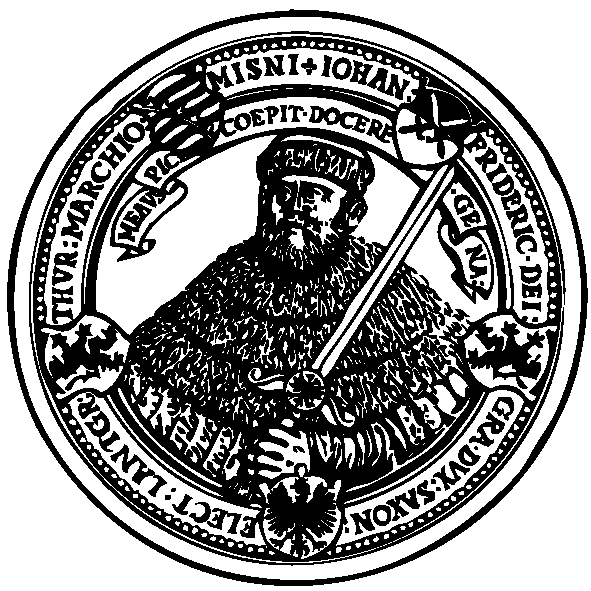
\includegraphics[height=6.0cm]{hanfriedTransparent}
  \end{center}
\end{frame}


\begin{frame}
  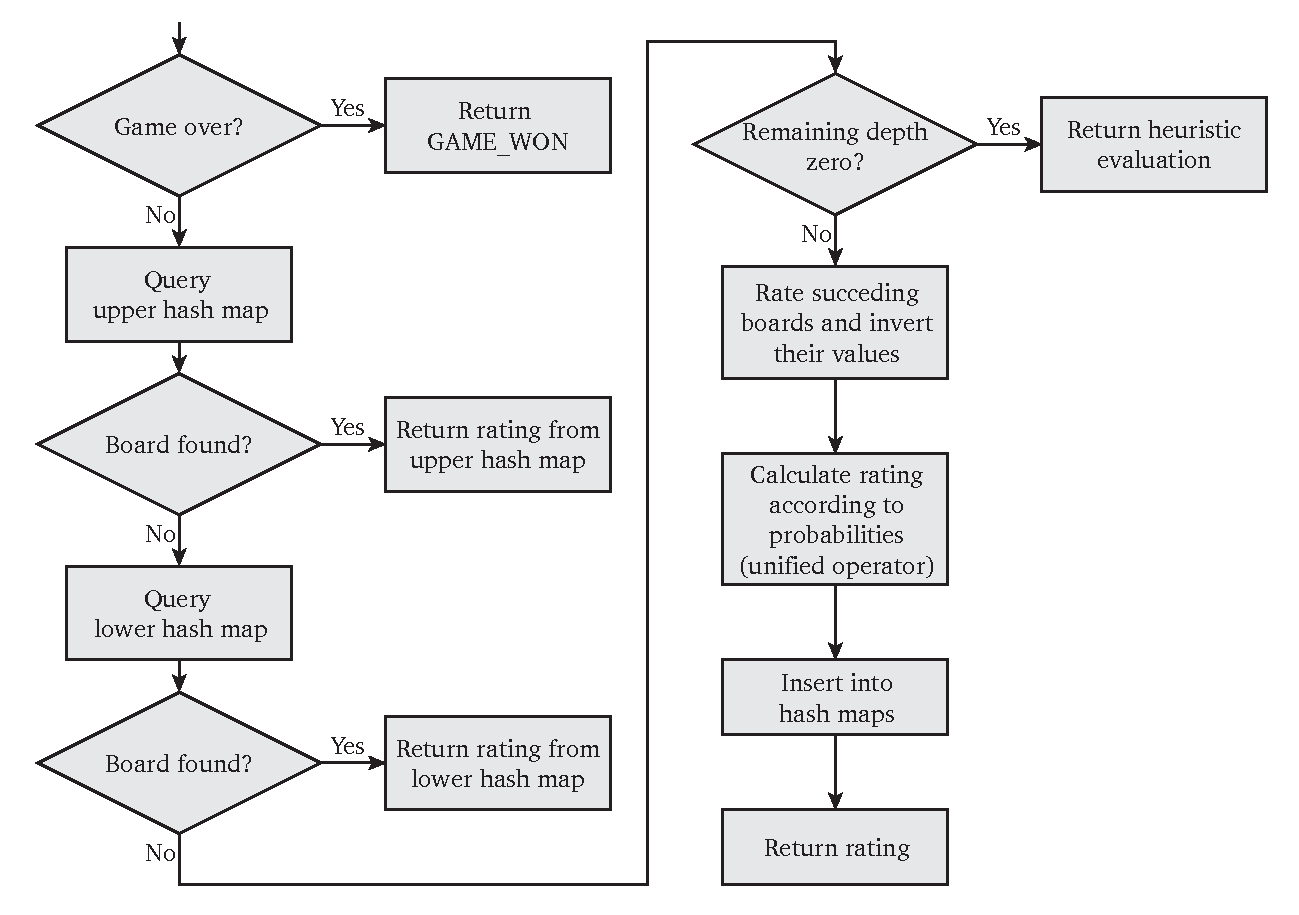
\includegraphics[scale=0.3]{treesearchImplementation}
\end{frame}

\end{document}

